\documentclass[table,11pt]{beamer}
\usepackage[brazil]{babel}
\usepackage[utf8]{inputenc} 
\usepackage[T1]{fontenc}
\usepackage[scaled=.90]{helvet}
\usepackage{courier}
\usepackage{url}
\usepackage{mathptmx}
\usepackage{mathtools}
\usepackage{listings}
\usepackage{bmpsize}
\usepackage{framed}
\usepackage{booktabs}
\usepackage{bookmark}
\usepackage{subfigure}
\usepackage{amsmath}
\usepackage{fancybox}
\usepackage{color}
\definecolor{oliveGreen}{rgb}{0, 0.50, 0} 
\definecolor{darkcerulean}{rgb}{0.03, 0.27, 0.49}
\usepackage{graphicx}
\usepackage[none]{hyphenat}
\usetheme{LES}
         
\title{Produção de Documentos e Apresentações com \LaTeX}
\author{Prof. Alcemir Rodrigues Santos}
\institute{\small Laboratório de Engenharia de Software\\[.25\baselineskip]
{\footnotesize Universidade Estadual do Piauí}}
\date{\today.}  

\begin{document} 
 
\begin{frame}[plain]    
  \titlepage  
\end{frame}   
    

\begin{frame}  
\frametitle{Outline} 
\tableofcontents
% You might wish to add the option [pausesections]
\end{frame} 

% 1.	Introdução com Breve história do LaTeX 
\section{Introdução}
\subsection{}

% =============== % 
%     Frame       % 
\begin{frame}
\frametitle{Breve História do \LaTeX}

\begin{itemize}
  \item Processador de textos $x$ Editor de textos
  \item \TeX (1977) -- Donald E. Knutch 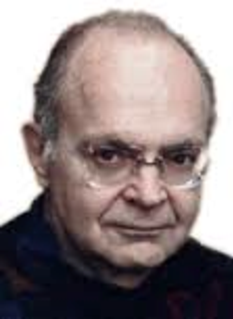
\includegraphics[scale=.4,keepaspectratio]{../img/knutch.pdf} 
  \item \LaTeX (1985) -- Leslie Lamport  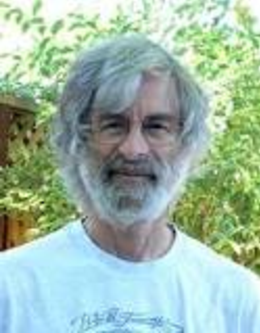
\includegraphics[scale=.4,keepaspectratio]{../img/lamport.pdf}
  \item \LaTeX $2_{\epsilon}$ (1994) -- LaTeX3 Team
\end{itemize}
\end{frame}


% =============== %
%     Frame       %
\begin{frame}
\frametitle{Por que usar \LaTeX?}

% You can create overlays
\begin{itemize}
  \item Conteúdo $x$ Formatação 
  \item Portabilidade
  \item Acabamento gráfico superior
  \item Estabilidade
  \item Escalabilidade
  \item Disponibilidade e custo
  \item Utilização de arquivos texto
  \item Suporte referências bibliográficas
  \item Fácil manejo de documentos grandes
\end{itemize}
 
\end{frame}

% =============== %
%     Frame       % 
\begin{frame}
\frametitle{Limitações \LaTeX?}

% You can create overlays
\begin{itemize}
  \item Personalização exige mais estudo
  \item São necessárias várias ferramentas 
  \item Legibilidade reduzida 
  \item Aprendizagem mais lenta
\end{itemize}
 
\end{frame}


% =============== %
%     Frame       %
\begin{frame}
\frametitle{Distribuições, Ajuda e Pacotes}

% You can create overlays
\begin{itemize}
  \item Distribuições para instalação 
  \begin{itemize}
    \item Unix/Linux (TeXLive): \url{http://www.tug.org/texlive/}
  	\item Windows (MikTeX): \url{http://www.miktex.org/}
  	\item MAC OS (MacTeX): \url{http://www.tug.org/mactex/}
  \end{itemize}

  \item Pessoas dispostas a ajudar
  \begin{itemize}
 	 \item \TeX~StackChange: \url{http://tex.stackexchange.com/}
  \end{itemize}
  
  \item Pacotes: arquivos e documentação
  \begin{itemize}
  	\item CTAN: \url{http://www.ctan.org/}
  \end{itemize}
\end{itemize}
 
\end{frame}


% =============== %
%     Frame       %
\begin{frame}
\frametitle{Livros para Estudo}

\begin{columns}
\column{.5\textwidth}

\includegraphics[scale=.15]{../img/livro1.pdf}  \textbf{LaTeX: A Documentation Preparation System}
Leslie Lamport e Duane Bibby 

 
\includegraphics[scale=.3]{../img/livro2.pdf}  \textbf{The LaTeX
Companion} Michel Goossens, Frank Mittelbach e Alexander Samarin 

\column{.5\textwidth}
	 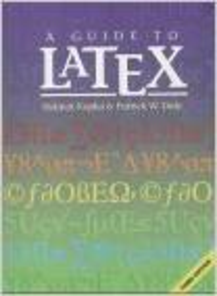
\includegraphics[scale=.3]{../img/livro3.pdf} \textbf{A Guide to LaTeX: Document Preparation for
Beginners and Advanced Users} Helmut Kopka e Patrick W. Daly 

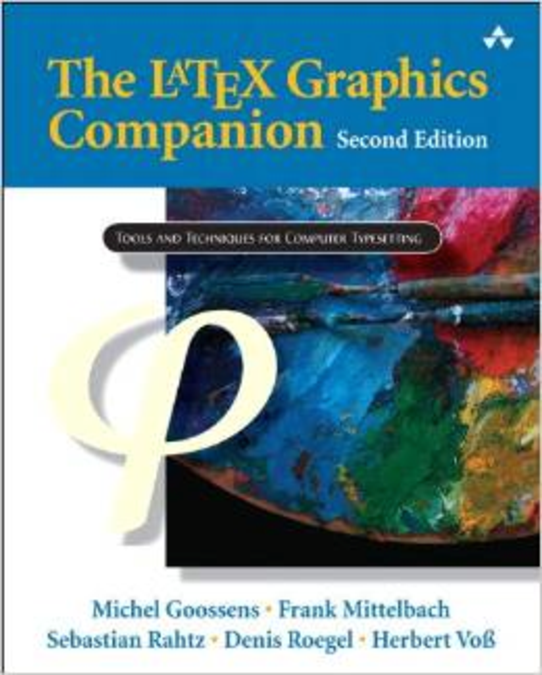
\includegraphics[scale=.15]{../img/livro4.pdf} \textbf{The LaTeX Graphics Companion} Michel Goossens,
Sebastian Rahtz e Frank Mittelbach
\end{columns}
 
\end{frame} 



% =============== %
%     Frame       %
\begin{frame}[fragile]
\frametitle{Estrutura lógica dos arquivos \LaTeX}
{\small
\begin{block}{Preâmbulo}
Tipos de documento, pacotes adicionais e comando gerais. 
\begin{verbatim}
	\documentclass[12pt,a4paper]{article}
	\usepackage{graphicx}
	\newcommand{\titulo}[1]{\large\bf #1}
	...
\end{verbatim}
\end{block}

\begin{block}{Corpo}
O texto do documento.
\begin{verbatim}
	\begin{document}
 	...
	\end{document}
\end{verbatim}
\end{block}
}
 
\end{frame}



% 2.	Criação de documentos (Estrutura, organização e construção)
\section{Documentos}

\subsection[]{Comandos Básicos}

% =============== %
%     Frame       %
\begin{frame}[fragile]
\frametitle{Notas}

\begin{itemize}
  \item Comandos: \verb|\command|, \verb|\command{}|, \verb|\command[]{}|
  \item Ambientes: \verb|\begin{ambiente}...\end{ambiente}|
  \item Caracteres especiais: \verb|$&%#_{}~^\| devem ser precedidos por \verb|\| ou o comando
  \verb|\verb|
  \item Espaçamento automático
  \item Comentários: usa-se o caractere \verb|%| ou \verb|\begin{comment}...\end{comment}|
  \item Delimitador de contexto: \verb|{ ... }|
  \item Referência a arquivos: \verb|/igual/ao/linux|
\end{itemize}
 
\end{frame}


% =============== %
%     Frame       %
\begin{frame}[fragile]
\frametitle{Exemplo funcional mínimo!}

\begin{block}{\LaTeX~hello world!}
\begin{verbatim}
	\documentclass[12pt,a4paper]{article}
	\begin{document}
		Hello world !
	\end{document}
\end{verbatim}
\end{block}
 
\end{frame}

% =============== %
%     Frame       %
\begin{frame}[fragile]
\frametitle{Detalhes do Exemplo}

\begin{block}{Opções}
\begin{verbatim} 
	10pt, 12pt, oneside, twoside, a4paper, 
	letterpaper, titlepage, twocolumn
\end{verbatim}
\end{block}
 \begin{block}{Documentos comuns}
\begin{verbatim} 
	article, book, report, slides, letter
\end{verbatim}
\end{block}
\end{frame}

% =============== %
%     Frame       %
\begin{frame}
\frametitle{O Processo de Compilação}


\begin{figure}
\centering
 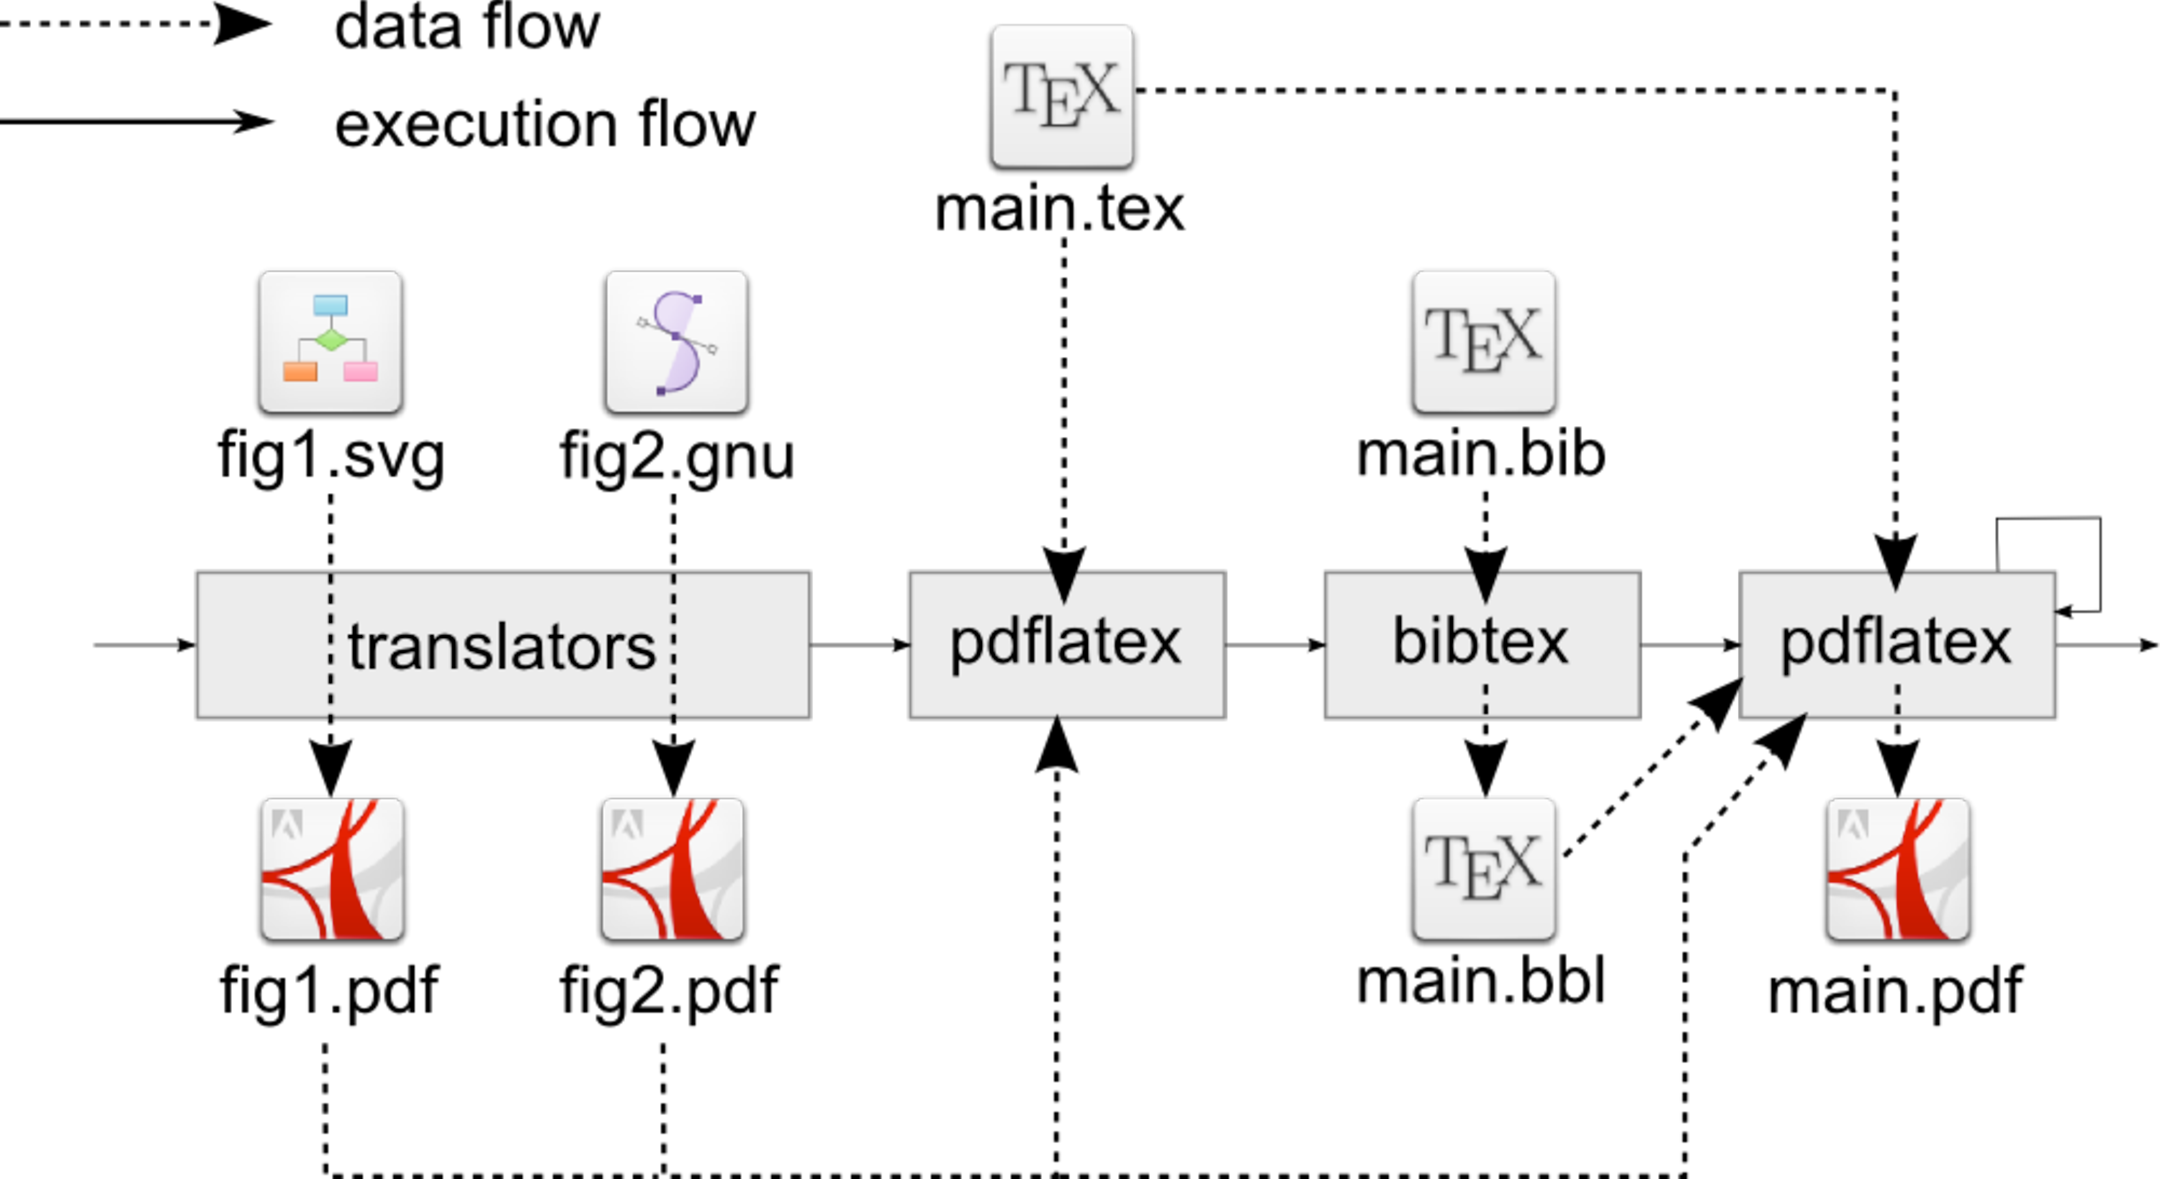
\includegraphics[scale=.25]{../img/process.pdf}
\end{figure}
 
\end{frame}

% =============== %
%     Frame       %
\begin{frame}[fragile]
\frametitle{}

% You can create overlays
\begin{itemize}
  \item O programa \texttt{latex} gera o arquivo \texttt{.dvi}: \texttt{latex arquivo.tex}
  \item A inclusão de referências bibliográficas feita através do programa \texttt{bibtex}:
  \texttt{bibtex arquivo}
  \item O \textit{PostScript} final pode ser gerado pelo \texttt{dvips}: \texttt{dvips arquivo.dvi
  -o arquivo.ps}
  \item O \textit{PostScript} pode ser visualizado e impressão pelo \texttt{gsview32.exe} (Windows)
  ou \texttt{gv} (Linux/Unix).
  \item Uma outra alternativa é utilizar o comando \texttt{pdflatex}
\end{itemize}
 
\end{frame}

% =============== %
%     Frame       %
\begin{frame}
\frametitle{Arquivos Comuns (1/2)}

\begin{itemize}
  \item \texttt{.tex}: Arquivos fontes
  \item \texttt{.log}: Relatório da compilação
  \item \texttt{.dvi}: Resultado da compilação dos arquivos fonte via \textit{latex}
  \item \texttt{.aux}: Arquivos auxiliar utilizado na geração documento final (\textit{.dvi} ou
  	\textit{.pdf})
  \item \texttt{.cls}: Arquivos de classe
  \item \texttt{.sty}: Pacotes
\end{itemize}
 
\end{frame}

% =============== %
%     Frame       % 
\begin{frame}
\frametitle{Arquivos Comuns (2/2)}

% You can create overlays
\begin{itemize}
  \item \texttt{.toc}: Itens para o sumário
  \item \texttt{.lof}: Itens para a lista de figuras
  \item \texttt{.lot}: Itens para a lista de tabelas
  \item \texttt{.bbl}: Itens para a lista de bibliografias
  \item \texttt{.blg}: Arquivos auxiliar utilizado na geração de bibliografias
\end{itemize}
 
\end{frame}


\subsection[]{Elaboração de documentos}\label{sec:elaboracao}
% =============== %
%     Frame       %
\begin{frame}[fragile]
\frametitle{Partes do Documento}

% You can create overlays
\begin{itemize}
  \item Tipos de divisões: \verb|\section{}|, \verb|\subsection{}|, \verb|\subsubsection{}|
\verb|\paragraph{}|, \verb|\subparagraph{}|
  \item Classe book: \verb|\part{}|, \verb|\chapter{}|
  \item Apêndices: \verb|\appendix|
\end{itemize}
 
\end{frame}

% =============== %
%     Frame       %
\begin{frame}[fragile]
\frametitle{Acentuando em Português}

% You can create overlays
\begin{itemize}
  \item Utilizar o pacote babel e fontes especiais: 
  \begin{verbatim}
  	\documentclass[12pt,a4paper]{article} 
  	\usepackage[latin1]{inputenc}
  	\usepackage[T1]{fontenc} 
  	\usepackage[brazil,english]{babel}
  	\begin{document} 
  	\selectlanguage{brazil}
  	...
  	\end{document}
  \end{verbatim}
\end{itemize}
 
\end{frame}

% =============== %
%     Frame       %
\begin{frame}[fragile]
\frametitle{Aplicando Formatações ao Texto}

% You can create overlays
\begin{itemize}
  \item Novo parágrafo: é suficiente deixar uma linha em branco 
  \item Negrito:  \verb|\textbf{text}| $\rightarrow$ \textbf{text}
  \item Itálico:  \verb|\textit{text}| $\rightarrow$ \textit{text}
  \item Texto centralizado, esquerda e direita: Usar ambientes \textit{center}, \textit{flushleft} e
 \textit{flushright}.
 \begin{verbatim}
     \begin{center}
     ... texto ...
     \end{center}
 \end{verbatim}
\end{itemize}
 
\end{frame}

% =============== %
%     Frame       %
\begin{frame}[fragile]
\frametitle{Gerando Listas}

% You can create overlays
\begin{itemize}
  \item Listas numeradas:
\end{itemize}
\begin{columns}
	\column{.5\textwidth}
\begin{verbatim}
	\begin{enumerate}
		\item Banana
		\item Batata
	\end{enumerate}
\end{verbatim}
	\column{.5\textwidth}
	\begin{framed}
	\begin{enumerate}
 		\item Banana
 		\item Batata
 	\end{enumerate}
	\end{framed}
\end{columns}
\end{frame}
	
	
% =============== %
%     Frame       %
\begin{frame}[fragile]
\frametitle{Gerando Listas}

% You can create overlays
\begin{itemize}
  \item Listas de itens:
\end{itemize}
\begin{columns}
	\column{.5\textwidth}
\begin{verbatim}
	\begin{itemize}
		\item Banana
		\item Batata
	\end{itemize}
\end{verbatim}
	\column{.5\textwidth}
	\begin{framed}
	\begin{itemize}
 		\item Banana
 		\item Batata
 	\end{itemize}
	\end{framed}
\end{columns}
\end{frame}


% =============== %
%     Frame       %
\begin{frame}[fragile]
\frametitle{Gerando Listas}

% You can create overlays
\begin{itemize}
  \item Listas de descrição:
\end{itemize}
\begin{columns}
	\column{.5\textwidth}
\begin{verbatim}
	\begin{description}
		\item[Fruta:] Banana
		\item[Ferramenta:] Martelo
	\end{description}
\end{verbatim}
	\column{.5\textwidth}
	\begin{framed}
	\begin{description}
		\item[Fruta:] Banana
		\item[Ferramenta:] Martelo
	\end{description}
	\end{framed}
\end{columns}
\end{frame}
	
% =============== %
%     Frame       %
\begin{frame}[fragile]
\frametitle{Edição Matemática Básica}

% You can create overlays
\begin{itemize}
  \item Modo texto $V.S$ modo matemático
  \item Separadores \verb|$ ... $| e \verb|$$ ... $$|: 
\end{itemize}
\begin{columns}
	\column{.5\textwidth}
\begin{verbatim}
	  Tem-se que $x=0$.
\end{verbatim}
	\column{.5\textwidth}
	\begin{framed}
	Tem-se que $x=0$.
	\end{framed}
\end{columns}
\begin{columns}
	\column{.5\textwidth}
\begin{verbatim}
	  Tem-se que: $$x=0$$.
\end{verbatim}
	\column{.5\textwidth}
	\begin{framed}
	Tem-se que: $$x=0$$.
	\end{framed}
\end{columns}

\end{frame}


% =============== %
%     Frame       %
\begin{frame}[fragile]
\frametitle{Edição Matemática Básica}

% You can create overlays
\begin{itemize}
  \item Sobrescrito e Subescrito:
      
\begin{columns}
\small
	\column{.6\textwidth}
\verb|$X^{sup}=Y_{inf}=Z^{sup}_{inf}$|
	\column{.4\textwidth}
	\begin{framed}
	$X^{sup}=Y_{inf}=Z^{sup}_{inf}$
	\end{framed}
\end{columns}

\item Espaços em modo matemático:
\begin{columns} \small
	\column{.6\textwidth}
	\verb|$a b,a\;b,a\;\;\;b$| 
	\column{.4\textwidth}
	\begin{framed}
	$a b,a\;b,a\;\;\;b$ 
	\end{framed}
\end{columns}

\item Negrito:
\begin{columns}\small
	\column{.6\textwidth}
\verb|$\mathbf{x} = [x_1 \;\; x_2]^T$|
	\column{.4\textwidth}
	\begin{framed}
	$\mathbf{x} = [x_1 \;\; x_2]^T$
	\end{framed}
\end{columns}
\end{itemize}
\end{frame}


% =============== %
%     Frame       %
\begin{frame}[fragile]
\frametitle{Edição Matemática Básica}

% You can create overlays
\begin{itemize}
  \item Vetores:
      
\begin{columns}
\small
	\column{.6\textwidth}
\begin{verbatim}
$$\vec{a},\hat{a},\bar{a},
\tilde{a},\dot{a},\ddot{a}$$
\end{verbatim}
	\column{.4\textwidth}
	\begin{framed}
	$$\vec{a},\hat{a},\bar{a},
	\tilde{a},\dot{a},\ddot{a}$$
	\end{framed}
\end{columns}

\item Somatórios e Integrais:
\begin{columns} \small
	\column{.6\textwidth}
	\begin{verbatim}
	$$\sum_{i=1}^{n}f(x_i)\Delta x 
	\approx \int_a^bf(x)dx$$
	\end{verbatim}
	\column{.4\textwidth}
	\begin{framed}
	 $$\sum_{i=1}^{n}f(x_i)\Delta x
	  \approx \int_a^bf(x)dx$$
	\end{framed}
\end{columns}

\end{itemize}
\end{frame}

% =============== %
%     Frame       %
\begin{frame}[fragile]
\frametitle{Edição Matemática Básica}

% You can create overlays
\begin{itemize}
	\item Frações:
	\begin{columns}
	\small
	\column{.6\textwidth}
	 \verb|$$(y+2)\frac{x+1}{x-1}$$|
	 \column{.4\textwidth}
	\begin{framed}
	$$(y+2)\frac{x+1}{x-1}$$
	\end{framed}	 
	 \end{columns}
	
	\item Limites e derivadas parciais: {\small
	\begin{verbatim}
$$\frac{\partial f(x,y)}{\partial x} =
\lim_{\Delta x \to 0}\frac{f(x+\Delta x,y)-
f(x,y)}{\Delta x}$$
	\end{verbatim}
	\begin{framed}
	$$\frac{\partial f(x,y)}{\partial x} =
\lim_{\Delta x \to 0}\frac{f(x+\Delta x,y)-
f(x,y)}{\Delta x}$$
	\end{framed}	
	}

\end{itemize}
 
\end{frame}
% =============== %
%     Frame       %
\begin{frame}[fragile]
\frametitle{Edição Matemática Básica}

% You can create overlays
\begin{itemize}
  \item Parênteses, chaves e colchetes:
  	\begin{columns}
	\small
	\column{.5\textwidth}
	\begin{verbatim}	
$$ \left[
   \left\{
     \left(
       {1 \over x}
     \right)^2 - 3
   \right\} + x^2
 \right]^3
 $$
	\end{verbatim}
	\column{.5\textwidth}
	\begin{framed}
	$$ \left[
   \left\{
     \left(
       {1 \over x}
     \right)^2 - 3
   \right\} + x^2
 \right]^3
 $$
	\end{framed}
 \end{columns}
\end{itemize}
 
\end{frame}

% =============== %
%     Frame       %
\begin{frame}[fragile]
\frametitle{Edição Matemática Básica}

% You can create overlays
\begin{itemize}
  \item Matrizes:  \textit{\color{oliveGreen}//Definição}
\begin{verbatim}
$$\mathbf{I} =
\left[
  \begin{array}{cccc}
  1      & 0      & \ldots & 0      \\
  0      & 1      & \ldots & 0      \\
  \vdots & \vdots & \ddots & \vdots \\
  0      & 0      & \ldots & 1
  \end{array}
\right]$$
\end{verbatim}
\end{itemize}
 
\end{frame}

% =============== %
%     Frame       %
\begin{frame}[fragile]
\frametitle{Edição Matemática Básica}

% You can create overlays
\begin{itemize}
  \item Matrizes:  \textit{\color{oliveGreen}//Resultado}
$$\mathbf{I} =
\left[
  \begin{array}{cccc}
  1      & 0      & \ldots & 0      \\
  0      & 1      & \ldots & 0      \\
  \vdots & \vdots & \ddots & \vdots \\
  0      & 0      & \ldots & 1
  \end{array}
\right]$$
\end{itemize}
 
\end{frame}

% =============== %
%     Frame       %
\begin{frame}[fragile]
\frametitle{Edição de Tabelas}


\begin{itemize}
  \item Ambiente \texttt{tabular}: {\color{oliveGreen} \textit{//Definição}}
 {\small
  \begin{verbatim}
\begin{tabular}{||l|c|c|r||} 
\hline
 Item & Preço & Quantidade & Total \\ 
\hline \hline
Banana & 0,55 & 5 & 2,75  \\
\hline
Batata & 0,35 & 3 & 1,05  \\
\hline \hline
       &      & Total & 3,80  \\
\hline
\end{tabular}  
  \end{verbatim}
 }
\end{itemize}
\end{frame}
% =============== %
%     Frame       %
\begin{frame}[fragile]
\frametitle{Edição de Tabelas}

\begin{itemize}
  \item Ambiente \texttt{tabular}: {\color{oliveGreen} \textit{//Resultado}}
  \newline
  \newline
\begin{tabular}{|l|c|c|r|} 
\hline
 Item & Preço & Quantidade & Total \\ 
\hline
Banana & 0,55 & 5 & 2,75  \\
\hline
Batata & 0,35 & 3 & 1,05  \\
\hline 
& & Total & 3,80 \\
\hline
\end{tabular}  
\end{itemize}
\end{frame}


% =============== %
%     Frame       %
\begin{frame}[fragile]
\frametitle{Incluindo Figuras}

\begin{itemize}
  \item Declarar o pacote \texttt{graphicx}: \verb|\usepackage{graphicx}|
  \item Inserir o comando \verb|\includegraphics[options]{path}|:
  \item Exemplo:
  {\small
  \begin{verbatim}
\includegraphics[scale=.3] {figs/leslie.ps}
  \end{verbatim}
  }
  \item Outras opções disponíveis: \textit{scale},\textit{width}, \textit{height} e \textit{angle}.
\end{itemize}
 
\end{frame}

% =============== %
%     Frame       %
\begin{frame}[fragile]
\frametitle{Mudando o tipo de fonte}

\begin{table}
\centering
\begin{tabular}{ll}
\toprule
\textbf{Comando} & \textbf{Família de fonte} \\
\midrule
\verb|\textit{Itálico}| & \textit{Itálico} \\
\verb|\textsc{Small Caps}| & \textsc{Small Caps} \\
\verb|\textbf{Negrito}| & \textbf{Negrito} \\
\verb|\texttt{Typewriter}| & \texttt{Typewriter} \\
\verb|\textsf{Sans Serif} | & \textsf{Sans Serif}\\
\verb|\textrm{Romano}| & \textrm{Romano} \\
\verb|\textsl{Inclinado}| & \textsl{Inclinado} \\
\bottomrule
\end{tabular}
\end{table}
 
\end{frame}

% =============== %
%     Frame       %
\begin{frame}[fragile]
\frametitle{Mudando o tamanho da fonte}

\begin{table}
\centering
\begin{tabular}{ll}
\toprule
\textbf{Comando} & \textbf{Tamanho resultante	} \\
\midrule
\verb|{\tiny LES}| &  {\tiny LES}\\
\verb|{\scriptsize LES}| & {\scriptsize LES} \\
\verb|{\footnotesize LES}| & {\footnotesize LES} \\
\verb|{\small LES}| & {\small LES} \\
\verb|{\normal LES}| & {\normal LES} \\
\verb|{\large LES}| & {\large LES} \\
\verb|{\Large LES}| & {\Large LES} \\
\verb|{\LARGE LES}| & {\LARGE LES} \\
\verb|{\huge LES}| & {\huge LES} \\
\verb|{\Huge LES}| & {\Huge LES} \\
\bottomrule
\end{tabular}
\end{table}
 
\end{frame}

% =============== %
%     Frame       %
\begin{frame}[fragile]
\frametitle{Estilo de Páginas}


\begin{itemize}
  \item O comando \verb|\pagestyle{}| define a aparência das páginas:
  \begin{itemize}
    \item \verb|\pagestyle{plain}|: Numeração no rodapé e sem cabeçalho.
    \item \verb|\pagestyle{headings}|: Numeração no rodapé e cabeçalho.
    \item \verb|\pagestyle{empty}|: Sem numeração ou cabeçalho.
    \item \verb|\pagestyle{myheadings}|: Permite que o usuário especifique através dos comandos
    \verb|\markboth{cab_esq}{cab_dir}| e \verb|\markright{cab_dir}|.
    \item Use \verb|\thispagestyle{estilo}| para mudar somente uma determinada página.
  \end{itemize}
\end{itemize}
 
\end{frame}

% =============== %
%     Frame       %
\begin{frame}[fragile]
\frametitle{Uma capa mínima e sumário}

\begin{itemize}
  \item Incluir \texttt{titlepage} nas opções de classe
  \item Definir o \textit{título} do trabalho, \textit{autor} e \textit{data}: 
\verb|\title{Curso de \LaTeX}|
\verb|\author{Alcemir Santos}|
\verb|\date{}|, \verb|\date{\today}| ou \verb|\date{Outubro/2008}|
  \item Colocar o comando \verb|\maketitle| depois do início do documento.
  \item Acrescentar a seguir o comando \verb|\tableofcontents|
\end{itemize}
 
\end{frame}
% =============== %
%     Frame       %
\begin{frame}[fragile]
\frametitle{Espaçamentos}

\begin{itemize}
	\item Horizontais:
	\item[] Efeito do comando \verb|\hspace{.83cm}|\hspace{.83cm} na linha
	\item[] Efeito do comando \verb|\hfill|\hfill na linha
	\item[] Efeito do comando \verb|\hrulefill|\hrulefill na linha
	\item[] Efeito do comando \verb|\dotfill|\dotfill na linha
	\item Verticais:
	\item[] Espaçamento fixo: \verb|\vspace{0.3cm}|\vspace{0.3cm}
	\item[] Preenchimento vertical: \verb|\vfill|\vfill
	\item \verb|\hspace*{}| e \verb|\vspace*{}| $\rightarrow$ evitam problemas com linha nova e página
nova
\end{itemize}
 
\end{frame}

% =============== %
%     Frame       %
\begin{frame}[fragile]
\frametitle{Mais formatação}

\begin{itemize}
  \item Se a hifenação falhar, colocar no preâmbulo: \verb|\hyphenation{hi-fen ma-nu-al}|
  \item O comando \verb|\pagebreak| inicia um nova página
  \item Notas de rodapé\footnote{como esta aqui em baixo.} podem ser feitas com
  \verb|\footnote{texto}|
\end{itemize}
 
\end{frame}

% =============== %
%     Frame       %
\begin{frame}[fragile]
\frametitle{Objetos Flutuantes}
\begin{columns}
	\small
	\column{.5\textwidth}
\begin{block}{Tabelas}
\begin{verbatim}
	\begin{table}[h|t|b|p]
\begin{tabular}
  ...
\end{tabular}
\end{table}
\end{verbatim}
\end{block}

	 \column{.5\textwidth}
\begin{block}{Figuras}
\begin{verbatim}
\begin{figure}[h|t|b|p] 
... 
\includegraphics{}
... 
\end{figure}
\end{verbatim}
\end{block}
\end{columns}

\begin{itemize}
  \item  \verb|\clearpage|
  \item[] Finaliza a página e força o aparecimento dos objetos flutuantes
  restantes
\end{itemize}
 
\end{frame}


% =============== %
%     Frame       %
\begin{frame}[fragile]
\frametitle{Multiplas Figuras}

Permite que várias figuras sejam agrupadas em uma só área.
    \begin{itemize}
    	\item \verb|\usepackage{subfigure}|
    \end{itemize}
    
\begin{verbatim}
\begin{figure}
\mbox{
    \subfigure[Caption (a)]{  
        \includegraphics[scale=.3]{fig-a.ps}  }
    \subfigure[caption (b)]{ 
        \includegraphics[scale=.3]{fig-b.ps}  }
}
\caption{Caption geral}
\end{figure}
\end{verbatim}

 
\end{frame}
% =============== %
%     Frame       %
\begin{frame}[fragile]
\frametitle{Algoritmos}

Permite a inclusão de arquivos com código\hyp{}fonte no documento, com formatação
  dependente da linguagem.
  \begin{verbatim}
  	\usepackage{listings}, \lstloadlanguages{C},
  	\lstset{language=C}, \lstinputlisting{filename}
  \end{verbatim}

\begin{framed}
\small
\begin{lstlisting}
#include <stdio.h>
/* Comment block */
int main(){
    // Line comment.
    printf("LaTeX is great for programmers!"));
    return 0;
}
\end{lstlisting} 
\end{framed}
\end{frame}

% =============== %
%     Frame       %
\begin{frame}[fragile]
\frametitle{Referências Cruzadas}

\begin{itemize}
  \item \verb|\label{ELEM-ID}|: Relaciona o elemento corrente do documento com a chave
  \texttt{ELEM-ID}.
  \item  Pode ser tabelas, figuras, seções, subseções, item de lista, \textit{etc}.
  \item \verb|\ref{ELEM-ID}|: Referencia o elemento relacionado com a chave \texttt{ELEM-ID}
  \item \verb|\pageref{ELEM-ID}|: Referencia a página onde está o elemento relacionado com
  a chave \texttt{ELEM-ID}
  \item As chaves devem ser únicas e são sensíveis à caixa
  \item Deve-se compilar duas vezes
\end{itemize}
 
\end{frame}


% =============== %
%     Frame       %
\begin{frame}[fragile]
\frametitle{Referências Cruzadas: tabelas}
{\scriptsize
\begin{columns}
\column{.5\textwidth}
\begin{verbatim}
\begin{table}
\centering
\begin{tabular}{|c|c|}\hline
Quant & R\$  \\ \hline
10    & 2.3  \\ \hline
\end{tabular}
\caption{Valores}
\label{tab:valores}
\end{table}

A Tabela~\ref{tab:valores} 
mostra \ldots
\end{verbatim}

\column{.5\textwidth}
\begin{table}
\centering
\begin{tabular}{|c|c|}\hline
Quant & R\$  \\ \hline
10    & 2.3  \\ \hline
\end{tabular}
\caption{Valores}
\label{tab:valores}
\end{table}

A Tabela~\ref{tab:valores} mostra \ldots
\end{columns}
 }
\end{frame}


% =============== %
%     Frame       %
\begin{frame}[fragile]
\frametitle{Referências Cruzadas: figuras}
{\scriptsize
\begin{columns}
\column{.5\textwidth}
\begin{verbatim}
\begin{figure}
\centering

\includegraphics[scale=.3]
   {./img/les}
\caption{LES.}
\label{fig:les}
\end{figure}
A Figura~\ref{fig:les} 
(Pág. \pageref{fig:les})
 mostra \ldots

A Figura~\ref{fig:les} 
mostra \ldots
\end{verbatim}

\column{.5\textwidth}
\begin{figure}
\centering

\includegraphics[scale=.3]{../img/les.pdf}
\label{fig:les}
\caption{LES }
\end{figure}
A Figura~\ref{fig:les} 
(Pág. \pageref{fig:les})
 mostra \ldots
\end{columns}
}
\end{frame}

% =============== %
%     Frame       %
\begin{frame}[fragile]
\frametitle{Referências Cruzadas: equações}
{\scriptsize
\begin{columns}
\column{.5\textwidth}
\begin{verbatim}
A Equação~\ref{eq:logn} mostra a definição
da  função logaritmo , válida
para $x>0$.

\begin{equation}
\ln(x)=\int_1^x
{1 \over t}dt
\label{eq:logn}
\end{equation}
\end{verbatim}

\column{.5\textwidth}
\begin{framed}
A Equação~\ref{eq:logn} mostra
a definição da função logaritmo,
válida para $x>0$.

\begin{equation}
\ln(x)=\int_1^x
{1 \over t}dt
\label{eq:logn}
\end{equation}
\end{framed}
\end{columns}
 }
\end{frame}

% =============== %
%     Frame       %
\begin{frame}[fragile]
\frametitle{Referências Cruzadas: equações}

Na início da seção adicionei o comando \verb|\label{}| após a definição da seção com
\verb|\section{}| assim:
\begin{verbatim}
\section{Minha seção} \label{sec:minha}
\end{verbatim}

A referência a esta seção deve ser feita assim:

\begin{columns}
\column{.5\textwidth}
\begin{verbatim}

A Seção \ref{sec:minha} 
apresenta \ldots

\end{verbatim}

\column{.5\textwidth}
\begin{framed}
A Seção \ref{sec:elaboracao}
apresenta \ldots
\end{framed}
\end{columns}
\end{frame}


% =============== %
%     Frame       %
\begin{frame}[fragile]
\frametitle{Referências Bibliográficas}

\begin{enumerate}
  \item Criar um arquivo de bibliografias (\textit{.bib})
  \item Utilizar o comando \verb|\cite{chave}| para indicar a referência bibliográfica desejada
  \item Definir o estilo de referência utilizada com \verb|\bibliographystyle{estilo}|
  \item Especificar o arquivo de bibliografias e o ponto de inserção com
  \verb|\bibliography{arquivo}|
  \item Utilizar o \texttt{bibtex}, compilador de referências
\end{enumerate}
 
\end{frame}

% =============== %
%     Frame       %
\begin{frame}[fragile]
\frametitle{Arquivo de Bibliográfias}

\begin{itemize}
  \item Formato:
  \begin{framed}
  \begin{verbatim}
	@tipo_de_citação{chave, 
	 campo_1 = {Valor 1},
	 campo_2 = {Valor 2},
	 ...,
     campo_n = {Valor n},
	}
  \end{verbatim}
  \end{framed}
  \item Tipos mais comuns: \textit{book}, \textit{article}, \textit{inproceedings},
  \textit{inbook}, \textit{masterthesis},
  \textit{phdthesis}, \textit{techreport}.
\end{itemize}
 
\end{frame}

% =============== %
%     Frame       %
\begin{frame}[fragile]
\frametitle{Citando Referências}


\begin{itemize}
  \item \verb|\cite{chave}|: coloca a chamada da referência e inclui na lista final
  \item \verb|\nocite{chave}|: não coloca a chamada mas inclui na lista
  \item \verb|\nocite{*}|: lista todas as referências bibliográficas sem chamada no texto
  \item[] 
  \item Leitura adicional: pacote \texttt{natbib}.
\end{itemize}
 
\end{frame}

% =============== %
%     Frame       %
\begin{frame}
\frametitle{Exercícios}


\begin{enumerate}
  \item Elaborar um documento com as estruturas vistas até aqui.
  \item Criar artigo com template\footnote{Disponível aqui: \url{http://bit.ly/1BQBTq9}} da
  Sociedade Brasileira de Computação.
\end{enumerate}
 
\end{frame}


% 3.	Criação de apresentações (Estrutura, organização e construção)
\section{Apresentações com Beamer}


\subsection[Estrutura]{Estrutura}
% =============== %
%     Frame       %
\begin{frame}
\frametitle{Sobre o Beamer}
\begin{itemize}
  \item Os comandos padrões e \LaTeXe\ também funcionam no Beamer
  \item Súmários podem ser gerados automáticamente
  \item Você pode facilmente criar efeitos dinâmicos
  \item A aparência pode ser mudada com uso de temas à seu gosto
  \item Os temas disponíveis por padrão são bem estruturados e fáceis de ler. O que torna a
  apresentação mais profissional e fácil da audiência seguir.
\end{itemize}
\end{frame}

% =============== %
%     Frame       %
\begin{frame}
\frametitle{Sobre o Beamer}
\begin{itemize}
  \item A aparência, cores e fontes utilizada na apresentação podem ser facilmente alterada de forma
  \textit{global}, mas alterações podem ser feitas de forma \textit{local}
  \item Você pode cirar apresentações usando o mesmo código utilizado no seu artigo \LaTeX
  \item A saída produzida é típicamente um \textcolor{darkcerulean}{\textit{.pdf} file}, o que
  facilita a apresentação em qualquer plataforma
  \item {\color{darkcerulean}Sua apresntação irá ter a mesma estrutua, independente de qual
  computador ou visualizador está sendo utilizado}
\end{itemize}
\end{frame}

\begin{frame}
\frametitle{Onde achar o Beamer?}
\begin{center}
Beamer está disponível para download \textcolor{darkcerulean}{\textit{gratuitamente}} em:\newline
\textcolor{darkcerulean}{\url{https://bitbucket.org/rivanvx/beamer/wiki/Home}}
\end{center}
\begin{center}
Existe bastante coisa sobre Beamer na Internet e existe também uma 
\textit{documentação} Beamer disponível no repositório acima e no endereço abaixo: \newline
\url{http://www.ctan.org/tex-archive/macros/latex/contrib/beamer/doc/}
\end{center}
\end{frame}


% =============== %
%     Frame       %
\begin{frame}
\frametitle{Usando templates prontos}
\begin{itemize}
  \item A maneira mais rápida de iniciar a desenvolver apresentações com Beamer é utilizar-se de
  templates prontos.
  \item Vários templates prontos estão disponíveis no repositório do Beamer
  \item Um exemplo pode ser encontrado seguindo este caminho:
  \url{beamer/solutions/conference-talks/conference-ornate-20min.en.tex}
  \item Copie o arquivo e modifique os conteúdos.
\end{itemize}
\end{frame}

% =============== %
%     Frame       %
\begin{frame}
\frametitle{Para testar suas apresentações}
\begin{itemize}
  \item Para ver como é uma apresentação, compile o código \LaTeX\ \textcolor{darkcerulean}{duas}
  vezes
  \item Abra o arquivo \textit{.pdf} com o visualizador disponível e utilize em modo ``Tela Cheia''
  \item O sumário gerado tem \textit{hyperlinks} nas seções e subseções, além de uma linha
  auxiliar com botões de navegação
\end{itemize}
\end{frame}

% =============== %
%     Frame       %
\begin{frame}[fragile]
\frametitle{Frames}
\scriptsize

\begin{itemize}
  \item  Cada projeto Beamer é feito de uma série de \textcolor{darkcerulean}{\textit{frames}}. Cada frame
produz um ou mais slides, dependendo da existência ou não de ``\textit{overlays}'', as quais serão
discutidas mais tarde.
  \item  A opção \verb|[plain]| causa a supressão de ``cabeçalho'', ``rodapé'', e ``barra lateral''.
  Útil pra exibir figuras grandes.

\end{itemize}
\begin{block}{Um frame básico}
	\verb|\begin{frame}[<alignment>]| \newline
  	\verb|\frametitle{Frame Title Goes Here}|\newline
	\verb|	Texto do frame e/ou o código LaTeX.|\newline
	\verb|\end{frame}|
\end{block} 
\end{frame}

% =============== %
%     Frame       %
\begin{frame}[fragile]
\frametitle{Frames}
\scriptsize
\begin{itemize}
  \item Para compor frames basta escrever seu texto ou código \LaTeX\ entre os
comandos \verb|\begin{}| e \verb|\end{}| frame.
  \item Os frames são centralizados \verb|[c]| por padrão. Os valores \verb|[t]| (alinhamento
superior) e \verb|[b]|  (alinhamento inferior) também são aceitos.
\end{itemize}

\begin{block}{Um frame básico}
	\verb|\begin{frame}[t]|\newline
  	\verb|\frametitle{Frame Title Goes Here}|\newline
	\verb|	Texto do frame e/ou o código LaTeX.|\newline
	\verb|\end{frame}|
\end{block}
\end{frame}

% =============== %
%     Frame       %
\begin{frame}[fragile]
\frametitle{``Capa'' para a apresentação }
O frame de capa mostra somente as informações inserida no início do documento:

\begin{block}{Um frame básico}
	\verb|\begin{frame}|\newline
  	\verb|   \titlepage|\newline
	\verb|\end{frame}|
\end{block}

\end{frame}


% =============== %
%     Frame       %
\begin{frame}[fragile]
\frametitle{``Capa'' para a apresentação }
Por padrão, o comando \verb|\titlepage| cria uma página que inclui:
\begin{itemize}
  \item Título
  \item Autor
  \item Afiliação
  \item Data
  \item Imagem (logo)
\end{itemize}

Caso algum desses valores não seja declarados no preâmbulo, eles não seram incluídos do slide de
capa.
\end{frame}


% =============== %
%     Frame       %
\begin{frame}[fragile]
\frametitle{Slide de Sumário}
O comando \verb|\tableofcontents| cria dinamicamente o sumário baseado na estrutura que você
definiu
 
\begin{block}{Slide de Sumário}
\scriptsize
	\verb|\begin{frame}|\newline
	\verb|  \frametitle{Sumário}|\newline
  	\verb|  \tableofcontents[ pausesections]|\newline
	\verb|\end{frame}|
\end{block}

Perceba que o argumento \texttt{pausesections} permite que os items apareçam seção à seção.
\end{frame}

% =============== %
%     Frame       %
\begin{frame}[fragile]
\frametitle{Juntando as coisas}
 
\begin{block}{Exemplo}
\scriptsize
	\verb|\begin{frame}|\newline
	\verb|  \titlepage|\newline
	\verb|\end{frame}|
	\newline
	\verb|\begin{frame}|\newline
	\verb|  \frametitle{Sumário}|\newline
  	\verb|  \tableofcontents[ pausesections]|\newline
	\verb|\end{frame}|\newline
	\newline
 	\verb|\begin{frame}|\newline
	\verb|  \frametitle{Introdução}|\newline
  	\verb|  Corpo do texto ou código LaTeX.|\newline
	\verb|\end{frame}|
\end{block}

\end{frame}


% =============== %
%     Frame       %
\begin{frame}[fragile]
\frametitle{Overlays}
\begin{itemize}
  \item \textit{Overlays} permitem que seus slides apareçam incrementalmente.
  \item Mais especificamente, em Beamer, \textcolor{darkcerulean}{overlays} controlam a ordem na
  qual as partes do frame aparecem.
  \item Uma maneira fácil de implementar overlays é usar o comando \verb|\pause| entre as partes que
  devem aparecer serparadamente
\end{itemize}
\end{frame}


% =============== %
%     Frame       %
\begin{frame}[fragile]
\frametitle{Overlays}
Por exemplo: 

\begin{verbatim}
\textbf{Step1:} Compute the maximal suffix of $w$
with respect to $\preceq_l$ (say $v$) and the
maximal suffix of $w$ with respect to $\preceq_r$
(say $v’$).
\pause

\textbf{Step 2:} Find words $u$, $u’$ such that
$w = uv = u’v’$.
\pause

\textbf{Step 3:} If $|v| \le |v’|$, then output
$(u,v)$. Otherwise, output$(u’,v’)$.
\end{verbatim}
\end{frame}

% =============== %
%     Frame       %
\begin{frame}[fragile]
\frametitle{Overlays (Resultado)}
\textbf{Step1:} Compute the maximal suffix of $w$
with respect to $\preceq_l$ (say $v$) and the
maximal suffix of $w$ with respect to $\preceq_r$
(say $v’$).
\pause

\textbf{Step 2:} Find words $u$, $u’$ such that
$w = uv = u’v’$.
\pause

\textbf{Step 3:} If $|v| \le |v’|$, then output
$(u,v)$. Otherwise, output$(u’,v’)$.
\end{frame}

% =============== %
%     Frame       %
\begin{frame}[fragile]
\frametitle{Especificação de Overlays}
São feitas com os símbolos ($<$, $>$) e indicam quais partes devem aparecer

A especificação \verb|<1->| diz ``mostre do slide 1 em diante.'' \verb|<1-3>| diz ``mostre do
slide 1 ao 3.'' \verb|<-3,5-6,8->| diz ``mostre todos os slides, exceto os slides 4 e 7.''

Um exemplo:
\begin{columns}
	\column{.5\textwidth}
	\small
\begin{verbatim}
	\begin{itemize}
   \item<1>    $abcadcabca$
   \item<1-2>  $abcabcabca$
   \item<1-2>  $accaccacca$
   \item<1>    $bacabacaba$
   \item<1,3>  $cacdaccacc$
   \item<1-2>  $caccaccacc$
\end{itemize}
\end{verbatim}
	\column{.5\textwidth}
	\small
\begin{itemize}
   \item<1>    $abcadcabca$
   \item<1-2>  $abcabcabca$
   \item<1-2>  $accaccacca$
   \item<1>    $bacabacaba$
   \item<1,3>  $cacdaccacc$
   \item<1-2>  $caccaccacc$
\end{itemize}\end{columns}

\end{frame}



% =============== %
%     Frame       %
\begin{frame}[fragile]
\frametitle{Especificação de Overlays}
Podem também ser utilizadas para dar efeito em partes do texto. Por exemplo, o código abaixo
aplica o comando \verb|\alert{}| somente nos slides especificados:

\begin{columns}
	\small
	\column{.6\textwidth}
\begin{verbatim}
\alert{Todos slides}
\alert<2>{Slide 2}
\alert<3>{Slide 3}
\alert<1,3>{Slides 1 e 3}
\alert<-2,4>{Slides 1, 2 e 4}
\end{verbatim} 
	\column{.4\textwidth}
	\alert{Todos slides}

\alert<2>{Slide 2}

\alert<3>{Slide 3}

\alert<1,3>{Slides 1 e 3}

\alert<-2,4>{Slides 1, 2 e 4}
\end{columns}
\vspace{.5cm}
\textbf{Nota:} Se quiser que cada item de uma lista apareça em ordem, basta usar a opção
\verb|[<+->]|. Exemplo: \verb|\begin{itemize}[<+->]|

\end{frame}


% =============== %
%     Frame       %
\begin{frame}[fragile]
\frametitle{Overlays em ambientes}

Overlays também podem ser utilizados em ambientes

\begin{columns}
	\column{.5\textwidth}
	\scriptsize
\begin{verbatim}
\begin{theorem}<1->
  Um teorema.
\end{theorem}

\begin{proof}<2->
  Uma prova.
\end{proof}
\end{verbatim}
	\column{.5\textwidth}
	\scriptsize
\begin{theorem}<1->
   Um teorema.
  \end{theorem}
  \begin{proof}<2->
   Uma prova.
  \end{proof}
\end{columns}

\end{frame}


% =============== %
%     Frame       %
\begin{frame}
\frametitle{Estrutura dos Frames}
Beamer provêm muitas formas de estruturar seus slides de forma que ele fiquem bem
organizados e fácil de sua audiência seguir. Como exemplos, temos:

\begin{itemize}
  \item Columns
  \item Blocks
  \item Boxes (Borders)
\end{itemize}
\end{frame}

% =============== %
%     Frame       %
\begin{frame}[fragile]
\frametitle{Estrutura dos Frames: Colunas}

O ambiente pode ser chamado como segue:

\begin{block}{}
\small
\verb|\begin{columns}|

\verb|  \column{.xx\textwidth}|

\verb|   Texto ou código da segunda coluna|

\verb|  \column{.xx\textwidth}|

\verb|   Texto ou código da segunda coluna|

\verb|\end{columns}|
\end{block}

Onde \alert{.xx} é porcentagem do slide. 
\end{frame}


% =============== %
%     Frame       %
\begin{frame}[fragile]
\frametitle{Estruturas dos Slides: Blocos}
Blocos podem ser utilizados para serparar uma porção específica do texto do restante do slide:

{\small
\begin{verbatim}
\begin{block}{Introdução à {\LaTeX}}
``Beamer é uma classe {\LaTeX} para criar
 apresentações\ldots''
\end{block}
\end{verbatim}
}

\begin{block}{Introdução à {\LaTeX}}
``Beamer é uma classe {\LaTeX} para criar apresentações\ldots''
\end{block}

\end{frame}


% =============== %
%     Frame       %
\begin{frame}[fragile]
\frametitle{Estruturas dos Slides: Blocos}
Outros ambientes podem ser utilizados como blocos:


\begin{block}{Introduction to {\LaTeX}}
\begin{tabular}{l|l}
\textbf{Conteúdo} & \textbf{Ambiente correspondente} \\
\hline
Genérico & \texttt{block}\\
Teoremas & \texttt{theorem}\\
Lemas & \texttt{lemma}\\
Provas & \texttt{proof}\\
Corolários & \texttt{corollary}\\
Exemplos & \texttt{example}\\
Título em destaque & \texttt{alertblock}\\
\end{tabular}
\end{block}

\end{frame}

% =============== %
%     Frame       %
\begin{frame}[fragile]
\frametitle{Estruturas dos Frames: Colunas e Blocos}

Podemos combinar ``colunas'' e ``blocos'' para fazer uma apresentação mais limpa.

\begin{verbatim}
\begin{columns}[t]
   \column{.5\textwidth}
       \begin{block}{Cabeçalho da Coluna 1}
          Corpo do texto da Coluna 1
       \end{block}
   \column{.5\textwidth}
       \begin{block}{Cabeçalho da Coluna 2}
          Corpo do texto da Coluna 2
       \end{block}
\end{columns}
\end{verbatim}

E temos como resultado\ldots
\end{frame}


% =============== %
%     Frame       %
\begin{frame}[fragile]
\frametitle{Estruturas dos Frames: Colunas e Blocos}


\begin{columns}[t]
   \column{.5\textwidth}
       \begin{block}{Cabeçalho da Coluna 1}
          Corpo do texto da Coluna 1
       \end{block}
   \column{.5\textwidth}
       \begin{block}{Cabeçalho da Coluna 2}
          Corpo do texto da Coluna 2
       \end{block}
\end{columns}
\vspace{1cm}

Perceba que a opção \verb|[t]| adicionado ao ambiente de colunas alinha os blocos por cima para que
eles fiquem na mesma linha vertical, diferentemente de centralizado no slide.
\end{frame}


% =============== %
%     Frame       %
\begin{frame}[fragile]
\frametitle{Estruturas dos Frames: Colunas e Blocos}

Bordas também podem ser utilizadas para adicionar uma organização à sua aprsentação. Com o uso do
pacote \texttt{fancybox} (lembre-se de declarar \verb|\usepackage{facybox}| no preâmbulo). 

\begin{block}{Borda de Textos}
\begin{tabular}{l|l}
\small
\textbf{Comando} & \textbf{Resultado} \\
\hline
\verb|\shadowbox{Texto}| & \shadowbox{Texto}\\
\verb|\fbox{Texto}| & \fbox{Texto}\\
\verb|\doublebox{Texto}| & \doublebox{Texto}\\
\verb|\ovalbox{Texto}| & \ovalbox{Texto}\\
\verb|\Ovalbox{Texto}| & \Ovalbox{Texto}\\
\end{tabular}
\end{block}
\end{frame}


\subsection[Aparência]{Aparência}


% =============== %
%     Frame       %
\begin{frame}[fragile]
\frametitle{Temas}
Temas podem mudar completamente a aparência de sua apresentação. Você escolhe o tema a ser
utilizados usando o comando \verb|\usetheme{}| com um dos seguintes argumentos:

\begin{block}{}
\centering
\begin{tabular}{cccc}
\small
\texttt{Antibes} & \texttt{Boadilla} & \texttt{Frankfurt} & \texttt{Juanlespins} \\
\texttt{Montpellier} & \texttt{Singapore} & \texttt{Bergen} & \texttt{Copenhagen} \\
\texttt{Goettingen} & \texttt{Madrid} & \texttt{Paloalto} & \texttt{Warsaw} \\
\texttt{Berkeley} & \texttt{Darmstadt} & \texttt{Hannover} & \texttt{Malmoe} \\
\texttt{Pittsburgh} & \texttt{Berlin} & \texttt{Dresden} & \texttt{Ilmenau} \\
\texttt{Marburg} & \texttt{Rochester} & & \\
\end{tabular}
\end{block}

\end{frame}


% =============== %
%     Frame       %
\begin{frame}[fragile]
\frametitle{Cores dos Temas}
Se você gosta do ``layout'' de um tema, mas não gosta da cor, você pode facilmente invocar uma nova
cor para o tema substituindo \texttt{default} no comando \verb|\usetheme{default}| inserido no
preâmbulo por um dos seguintes argumentos:

\begin{block}{}
\centering
\begin{tabular}{cccc}
\small
\texttt{albatross} & \texttt{crane} & \texttt{beetle} & \texttt{dove} \\
\texttt{fly} & \texttt{seagull} & \texttt{wolverine} & \texttt{beaver} \\
\end{tabular}
\end{block}

\end{frame}



% =============== %
%     Frame       %
\begin{frame}[fragile]
\frametitle{Cores dos Temas}
Existe também a possibilidade de especificar cores para a parte \textit{interna} ou
\textit{externa} da mesma forma da cor geral do tema: substituindo \texttt{default} no comando
\verb|\usetheme{default}|.


\begin{columns}[t]
   \column{.5\textwidth}
       \begin{block}{Opções parte interna}
          \centering
\begin{tabular}{ccc}
\small
\texttt{lily} & \texttt{orchid} & \texttt{rose} \\
\end{tabular}
       \end{block}
   \column{.5\textwidth}
       \begin{block}{Opções parte externa}
                    \centering
\begin{tabular}{ccc}
\small
\texttt{whale} & \texttt{seahorse} & \texttt{dolphin} \\
\end{tabular}
       \end{block}
\end{columns}

\end{frame}


% =============== %
%     Frame       %
\begin{frame}
\frametitle{Exercício}

% You can create overlays
\begin{enumerate}
  \item Elaborar uma apresentação com as estruturas vistas.
\end{enumerate}
 
\end{frame}


% 4.	Links Úteis e Ajuda
\section{Conslusão}

\begin{frame}
\frametitle{Nota sobre o material} 

\begin{itemize}
  \item Este material foi criado com base em duas referencias principais:
  \begin{itemize}
		\item Curso de extensão em \LaTeX mistrado por \textit{Messias Alves} em 2008.
    {\color{darkcerulean} /*Parte sobre a criação de documentos*/}
		\item Tutorial de Beamer em Beamer, do \textit{Prof. Charles T. Batts} de
		2007. {\color{darkcerulean} /*Parte sobre a criação de apresentações*/}
  \end{itemize}
\end{itemize}
\end{frame}


\begin{frame}
\frametitle{Links Úteis} 

\begin{itemize}
  \item \url{http://latex.simon04.net/}
  \item \url{http://deic.uab.es/~iblanes/beamer_gallery/index_by_theme.html}
  \item \url{http://texdoc.net/texmf-dist/doc/latex/beamer/doc/beameruserguide.pdf}
  \item \url{http://www.stdout.org/~winston/latex/latexsheet.pdf}
  \item \url{http://en.wikibooks.org/wiki/LaTeX}
  \item {\Large \color{darkcerulean} \url{http://tex.stackexchange.com/}}
\end{itemize}
\end{frame}


\begin{frame}
\frametitle{Obrigado}

Happy \LaTeX\ coding!

Obrigado por ter tirado um tempo para estar aqui e acompanhar este tutorial de \LaTeX\. Agora você
deve ter um conhecimento básico para começar a criar seus documentos e apresentações com alta
qualidade.
\begin{figure}

\includegraphics[scale=.05]{../img/thank-you}
\end{figure}

\end{frame}



\end{document} 
